\documentclass{article} % Document class

% Packages
\usepackage[utf8]{inputenc} % Input encoding
\usepackage[T1]{fontenc}    % Output encoding
\usepackage{booktabs}
\usepackage{enumitem}
\usepackage{amssymb}
\usepackage{xcolor}
\usepackage{listings}
\usepackage{graphicx} % insert picture
\usepackage{hyperref}
\usepackage{array} % adjust table space


\definecolor{github-light-bg}{RGB}{255, 255, 255}
\definecolor{github-light-fg}{RGB}{3, 102, 214}
\definecolor{github-light-yellow}{RGB}{128, 102, 0}
\definecolor{github-light-orange}{RGB}{170, 0, 17}
\definecolor{github-light-purple}{RGB}{102, 51, 153}
\definecolor{github-light-cyan}{RGB}{0, 128, 128}
\definecolor{github-light-green}{RGB}{0, 128, 0}
\definecolor{github-light-red}{RGB}{204, 0, 0}

\lstdefinestyle{githublight}{
	backgroundcolor=\color{github-light-bg},
	basicstyle=\color{github-light-fg}\ttfamily,
	commentstyle=\color{github-light-green},
	keywordstyle=\color{github-light-purple},
	numberstyle=\tiny\color{github-light-fg},
	stringstyle=\color{github-light-cyan},
	identifierstyle=\color{github-light-orange},
	emphstyle=\color{github-light-red},
	emph={[2]TRUE,FALSE},
	emphstyle={[2]\color{github-light-yellow}},
	breaklines=true,
	breakatwhitespace=true,
	numbers=left,
	numbersep=5pt,
	stepnumber=1,
	showstringspaces=false,
	frame=single,
	rulecolor=\color{github-light-fg},
	framerule=0.5pt,
	tabsize=4,
	columns=flexible,
	extendedchars=true,
	inputencoding=utf8,
	upquote=true,
}

\lstset{style=githublight}

% Page layout settings
\usepackage[a4paper, margin=2.5cm]{geometry} % Set paper size and margins


\newcommand{\Sref}[1]{Section~\ref{#1}}
\newtheorem{hyp}{Hypothesis}

\title{Problem Set 2}
\date{Due: February 18, 2024}
\author{Applied Stats II}


\begin{document}
	\maketitle
	\section*{Instructions}
	\begin{itemize}
		\item Please show your work! You may lose points by simply writing in the answer. If the problem requires you to execute commands in \texttt{R}, please include the code you used to get your answers. Please also include the \texttt{.R} file that contains your code. If you are not sure if work needs to be shown for a particular problem, please ask.
		\item Your homework should be submitted electronically on GitHub in \texttt{.pdf} form.
		\item This problem set is due before 23:59 on Sunday February 18, 2024. No late assignments will be accepted.
		\item Total available points for this homework is 80.
	\end{itemize}

	
	\vspace{.25cm}
	
\noindent In this problem set, you will run several regressions and create an add variable plot (see the lecture slides) in \texttt{R} using the \texttt{incumbents\_subset.csv} dataset. Include all of your code.

	\vspace{.25cm}
\section*{Question 1} %(20 points)}
\vspace{.25cm}
\noindent We're interested in what types of international environmental agreements or policies people support (\href{https://www.pnas.org/content/110/34/13763}{Bechtel and Scheve 2013)}. So, we asked 8,500 individuals whether they support a given policy, and for each participant, we vary the (1) number of countries that participate in the international agreement and (2) sanctions for not following the agreement. \\

\noindent Load in the data labeled \texttt{climateSupport.RData} on GitHub, which contains an observational study of 8,500 observations.

\begin{itemize}
	\item
	Response variable: 
	\begin{itemize}
		\item \texttt{choice}: 1 if the individual agreed with the policy; 0 if the individual did not support the policy
	\end{itemize}
	\item
	Explanatory variables: 
	\begin{itemize}
		\item
		\texttt{countries}: Number of participating countries [20 of 192; 80 of 192; 160 of 192]
		\item
		\texttt{sanctions}: Sanctions for missing emission reduction targets [None, 5\%, 15\%, and 20\% of the monthly household costs given 2\% GDP growth]
		
	\end{itemize}
	
\end{itemize}

\newpage
\noindent Please answer the following questions:

\begin{enumerate}
	\item
	Remember, we are interested in predicting the likelihood of an individual supporting a policy based on the number of countries participating and the possible sanctions for non-compliance.
\begin{enumerate}
		\item Fit an additive model. Provide the summary output, the global null hypothesis, and $p$-value. Please describe the results and provide a conclusion.
		\item How many iterations did it take to find the maximum likelihood estimates?
	\end{enumerate}
	
	\item
	If any of the explanatory variables are significant in this model, then:
	\begin{enumerate}
		\item
		For the policy in which nearly all countries participate [160 of 192], how does increasing sanctions from 5\% to 15\% change the odds that an individual will support the policy? (Interpretation of a coefficient)
		\item
		For the policy in which very few countries participate [20 of 192], how does increasing sanctions from 5\% to 15\% change the odds that an individual will support the policy? (Interpretation of a coefficient)
		\item
		What is the estimated probability that an individual will support a policy if there are 80 of 192 countries participating with no sanctions? 
		\item
		Would the answers to 2a and 2b potentially change if we included the interaction term in this model? Why? 
		\begin{itemize}
			\item Perform a test to see if including an interaction is appropriate.
		\end{itemize}
	\end{enumerate}
\end{enumerate}
\vspace{1.5cm}
\noindent 	1. Remember, we are interested in predicting the likelihood of an individual supporting a policy based on the number of countries participating and the possible sanctions for non-compliance.\\

\noindent (a).  Fit an additive model. Provide the summary output, the global null hypothesis, and $p$-value. Please describe the results and provide a conclusion.\\

\lstinputlisting[language=R, firstline=42,lastline=67]{PS02_answers_Chenxi.R} 
\newpage
\begin{table}[h] \centering   \caption{Outcome variable is \texttt{choice} and the explanatory variables are \texttt{countries} and \texttt{sanctions}}   \label{} \begin{tabular}{@{\extracolsep{5pt}}lc} 
\\[-1.8ex]\hline \hline \\[-1.8ex]  & \multicolumn{1}{c}{\textit{Dependent variable:}} \\ \cline{2-2} \\[-1.8ex] & choice \\ \hline \\[-1.8ex]  countries80 of 192 & 0.336$^{***}$ \\   & (0.054) \\  
countries160 of 192 & 0.648$^{***}$ \\   & (0.054) \\   
sanctions5\% & 0.192$^{***}$ \\   & (0.062) \\   
sanctions15\% & $-$0.133$^{**}$ \\   & (0.062) \\   
sanctions20\% & $-$0.304$^{***}$ \\   & (0.062) \\   
Constant & $-$0.273$^{***}$ \\   & (0.054) \\  
\hline \\[-1.8ex] Observations & 8,500 \\ Log Likelihood & $-$5,784.130 \\ Akaike Inf. Crit. & 11,580.260 \\ \hline \hline \\[-1.8ex] \textit{Note:}  & \multicolumn{1}{r}{$^{*}$p$<$0.1; $^{**}$p$<$0.05; $^{***}$p$<$0.01} \\ 
\end{tabular} 
\end{table}  

\noindent There is a \textbf{positive} and statistically reliable relationship between the \texttt{choice} and the levels 80 of 192, 160 of 192 in \texttt{countries}, and the level  5\% in \texttt{sanctions}. There is a \textbf{negative} and statistically reliable relationship between the \texttt{choice} and the level 15\%, 20\% in \texttt{sanctions}.\\
Below is the description under certain level of sanctions situations:
\begin{itemize}
	\item For a certain level of sanctions, few countries participate [20 of 192] \textbf{decreases} the \textbf{log odds} of individual support 0.273 (the constant).
	\item For a certain level of sanctions, some countries participate [80 of 192] \textbf{increases} the \textbf{log odds} of individual support 0.336.
	\item For a certain level of sanctions, most countries participate [160 of 192] \textbf{increases} the \textbf{log odds} of individual support 0.648.
\end{itemize}
Below is the description under certain level of participate countries situations
\begin{itemize}
	\item For a certain level of participate countries, none sanction \textbf{decreases} the \textbf{log odds} of individual support 0.273 (the constant).
	\item For a certain level of participate countries, 5\% sanction \textbf{increases} the \textbf{log odds} of individual support 0.192.
	\item For a certain level of participate countries, 15\% sanction \textbf{decreases} the \textbf{log odds} of individual support 0.133.
	\item For a certain level of participate countries, 20\% sanction \textbf{decreases} the \textbf{log odds} of individual support 0.304.
\end{itemize}

\newpage

\noindent The global null hypothesis is: \\
\begin{center}
	$H_0: \beta_1 = \beta_2 = \beta_3 = ... = \beta_p = 0$ \\
	$H_1$: at least one slope is not equal to 0 \\
\end{center}

\lstinputlisting[language=R, firstline=71,lastline=80]{PS02_answers_Chenxi.R} 

\noindent And we get the outputs:

\begin{verbatim}
	Analysis of Deviance Table
	Model 1: choice ~ 1
	Model 2: choice ~ countries + sanctions  
	Resid. Df Resid. Dev Df Deviance  Pr(>Chi)    
	1      8499      11783                          
	2      8494      11568  5   215.15 < 2.2e-16 ***
	---
	Signif. codes:  0 ‘***’ 0.001 ‘**’ 0.01 ‘*’ 0.05 ‘.’ 0.1 ‘ ’ 1
\end{verbatim}

\noindent We can see that the p-value (< 2.2e - 16) is below the $\alpha$ = 0.05 threshold, so we would say that we find sufficient evidence to reject the null hypothesis. So, we know at least one slope is not equal to 0.\\

\vspace{.5cm}
\noindent (b). How many iterations did it take to find the maximum likelihood estimates?\\

\noindent In our logistic regression model summary, we will find an outputs like: \\
\lstinputlisting[language=R, firstline=66,lastline=67]{PS02_answers_Chenxi.R} 
\begin{verbatim}
	Number of Fisher Scoring iterations: 4
\end{verbatim}
So, it takes 4 iterations to find the maximum likelihood estimate.

\newpage

\noindent 2.If any of the explanatory variables are significant in this model, then:\\

\noindent In Question 1, we know the formula of this module is:

\begin{center}
$logit(p_{choice}) = -0.273 + 0.336 contries[80/192] + 0.648 countries[160/192] + 0.192 sanctions[5\%] - 0.133 sanctions[15\%] - 0.304 sanctions [20\%]$
\end{center}
\noindent (a).For the policy in which nearly all countries participate [160 of 192], how does increasing sanctions from 5\% to 15\% change the odds that an individual will support the policy? (Interpretation of a coefficient)\\

\noindent We know the countries level is [160 of 192], then we can write two formulas to present the 5\% sanctions situation and 15\% sanctions situation: \\
\begin{center}
$logit(p_{choice}) = -0.273 + 0.648 * 1 + 0.192 * 1 ............ (1) $\\
$logit(p_{choice}) = -0.273 + 0.648 * 1 - 0.133 * 1 ............  (2) $ \\
$(2) - (1) = \Delta logit(p_{choice}) = 0.242 - 0.567 =  - 0.325 $\\
$odd\ \ ratios =  e ^ {(-0.325)} \approx 0.723 $
\end{center}

\noindent So, we can know: If a policy is nearly all countries participate [160 of 192], increased sanctions from 5\% to 15\% will increase odds of individual agree with the policy by a multiplicative factor of 0.723. \\

\noindent (b).For the policy in which very few countries participate [20 of 192], how does increasing sanctions from 5\% to 15\% change the odds that an individual will support the policy? (Interpretation of a coefficient)\\

\noindent We know the countries level is [20 of 192], then we can write two formulas to present the 5\% sanctions situation and 15\% sanctions situation: \\
\begin{center}
	$logit(p_{choice}) = -0.273 + 0.192 * 1 ............ (1) $\\ 
	$logit(p_{choice}) = -0.273 - 0.133 * 1 ............  (2) $ \\ 
	$(2) - (1) = \Delta logit(p_{choice}) = -0.406 - (- 0.081) = -0.325$\\
	$odd\ \ ratios =  e ^ {(-0.325)} \approx 0.723 $
\end{center}

\noindent So, we can know: If a policy is very few countries participate [20 of 192], increased sanctions from 5\% to 15\% will increase odds of individual agree with the policy by a multiplicative factor of 0.723. \\

\noindent (c).What is the estimated probability that an individual will support a policy if there are 80 of 192 countries participating with no sanctions? \\

\noindent We know the countries level is [80 of 192], and the sanctions level is none, then we can write the formula: \\
\begin{center}
	$logit(p_{choice}) = -0.273 + 0.336 = 0.063$\\ 
\end{center}
\noindent And we know the formula is: 
\begin{center}
	$ P = \frac{1} { 1 + e^{-logit(P)}}$ ->
	$ P = \frac{1} { 1 + e^{-0.063}}$ ->
	$P \approx 0.516 $\\
\end{center}

\noindent And we can use predict code in \texttt{R} to check again:
\lstinputlisting[language=R, firstline=82,lastline=87]{PS02_answers_Chenxi.R} 

\begin{verbatim}
	 1 
	 0.5159191 
\end{verbatim}

So, we can conclude that if there are 80 out of 192 countries participating with no sanctions, the estimated probability will be approximately 0.516 on average. \\

\newpage 
\noindent (d).Would the answers to 2a and 2b potentially change if we included the interaction term in this model? Why? \\

\noindent The answers will not change. Because we didn't find enough evidence that including an interactive effect of \texttt{countries} and \texttt{sanctions} is a significant predictor for odds of deciding in individual policy support choice. Below is the process: \\

\lstinputlisting[language=R, firstline=89,lastline=93]{PS02_answers_Chenxi.R} 

\begin{table}[!htbp] \centering   \caption{Outcome variable is \texttt{choice} and explanatory variables are \texttt{countries}, \texttt{sanctions} and interaction}   \label{} 
\begin{tabular}{@{\extracolsep{5pt}}lc} \\[-1.8ex]\hline \hline \\[-1.8ex]  & \multicolumn{1}{c}{\textit{Dependent variable:}} \\ \cline{2-2} \\[-1.8ex] & choice \\ \hline \\[-1.8ex]  
countries80 of 192 & 0.376$^{***}$ \\   & (0.106) \\   
countries160 of 192 & 0.613$^{***}$ \\   & (0.108) \\   
sanctions5\% & 0.122 \\   & (0.105) \\   
sanctions15\% & $-$0.097 \\   & (0.108) \\    
sanctions20\% & $-$0.253$^{**}$ \\   & (0.108) \\   
countries80 of 192:sanctions5\% & 0.095 \\   & (0.152) \\   
countries160 of 192:sanctions5\% & 0.130 \\   & (0.151) \\   
countries80 of 192:sanctions15\% & $-$0.052 \\   & (0.152) \\   
countries160 of 192:sanctions15\% & $-$0.052 \\   & (0.153) \\   
countries80 of 192:sanctions20\% & $-$0.197 \\   & (0.151) \\   
countries160 of 192:sanctions20\% & 0.057 \\   & (0.154) \\   
Constant & $-$0.275$^{***}$ \\   & (0.075) \\  
\hline \\[-1.8ex] Observations & 8,500 \\ Log Likelihood & $-$5,780.983 \\ Akaike Inf. Crit. & 11,585.970 \\ \hline \hline \\[-1.8ex] \textit{Note:}  & \multicolumn{1}{r}{$^{*}$p$<$0.1; $^{**}$p$<$0.05; $^{***}$p$<$0.01} \\ 
\end{tabular}
\end{table} 

\noindent The global null hypothesis is: \\
\begin{center}
	$H_0: \beta_1 = \beta_2 = \beta_3 = ... = \beta_p = 0$ \\
	$H_1$: at least one slope is not equal to 0 \\
\end{center}

\lstinputlisting[language=R, firstline=95,lastline=98]{PS02_answers_Chenxi.R} 

\noindent And we get the outputs:\\

\begin{verbatim}
Analysis of Deviance Table

Model 1: choice ~ 1Model 
2: choice ~ countries * sanctions  
Resid. Df Resid. Dev Df Deviance  Pr(>Chi)    
1      8499      11783                          
2      8488      11562 11   221.44 < 2.2e-16 ***
---
Signif. codes:  0 ‘***’ 0.001 ‘**’ 0.01 ‘*’ 0.05 ‘.’ 0.1 ‘ ’ 1
\end{verbatim}

\noindent We can see that the p-value (< 2.2e - 16) is below the $\alpha$ = 0.05 threshold, so we would say that we find sufficient evidence to reject the null hypothesis. So, we know at least one slope is not equal to 0.\\

\noindent And we can make a significant test for different slopes.

\begin{center}
	$H_0:  \beta_{\# of countries | sanctions} = \beta_{\# of countries | sanctions}$ \\
	$H_1: $ Effect of countries participate is different by sanctions levels. \\
\end{center}
\lstinputlisting[language=R, firstline=103,lastline=104]{PS02_answers_Chenxi.R} 

\begin{verbatim}
	Analysis of Deviance Table
	
	Model 1: choice ~ countries + sanctions
	Model 2: choice ~ countries * sanctions  
	Resid. Df Resid. Dev Df Deviance Pr(>Chi)
	1      8494      11568                     
	2      8488      11562  6   6.2928   0.3912
\end{verbatim}

\noindent We can see that the p-value (0.3912) is upper the $\alpha$ = 0.05 threshold, so, there is not evidence that including an interactive effect of \texttt{countries} and \texttt{sanctions} is a significant predictor for odds of deciding in individual policy support choice.\\

And we can also visualize these two models scatter to see details:\\

\lstinputlisting[language=R, firstline=106,lastline=137]{PS02_answers_Chenxi.R} 

\begin{figure}[h]
	\centering
	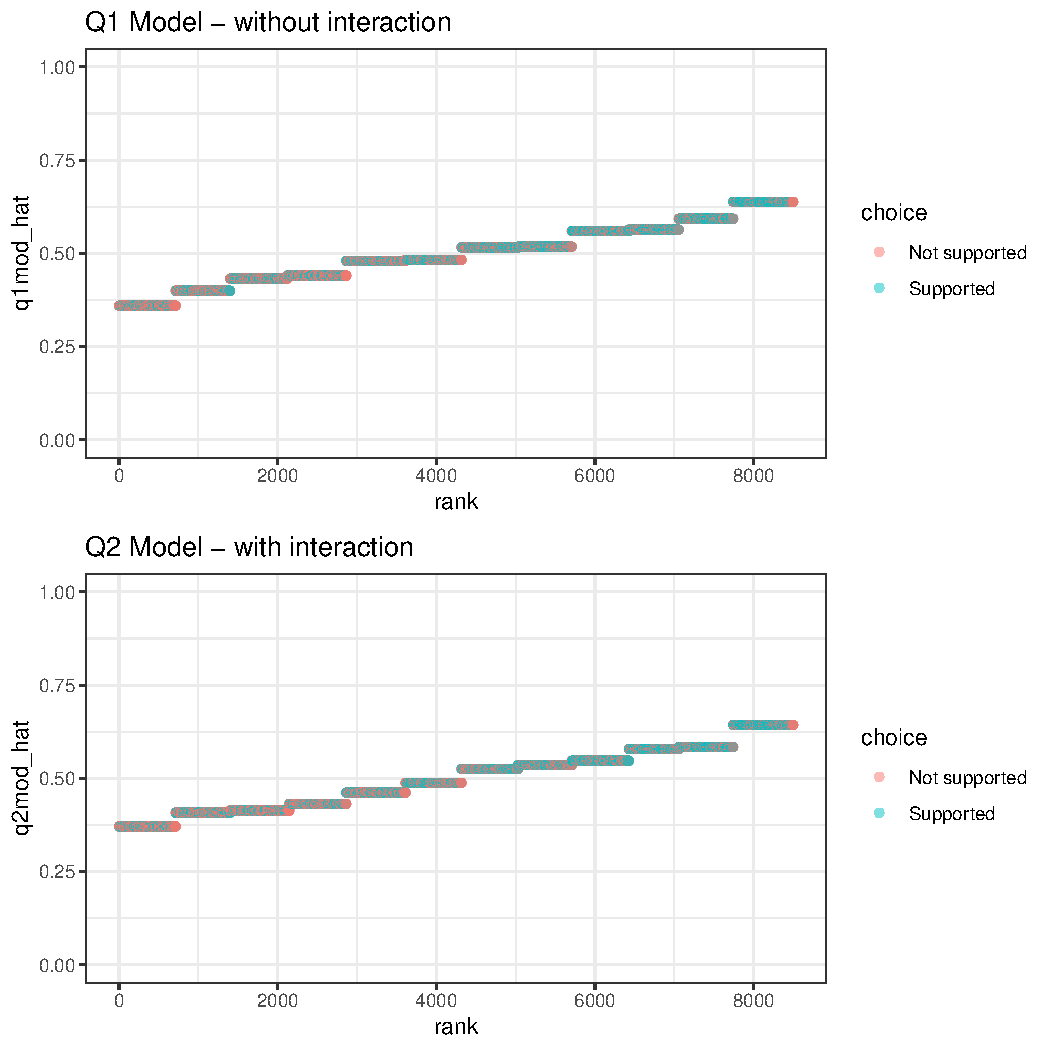
\includegraphics[scale=1]{q2_plot1.pdf} 
	\caption{Scatter - Model 1 and Model 2}
\end{figure}

\end{document}
